% @author Benjamin Schröder
%
% Quellen: 5, 9, 10, 14, 15, 16, 17, 18, 19, 24, 25
%
% 5:
%   - Definition von PCG
%   - Vorstellen von einigen Verfahren
%
% 9:
%   - Definition von PCG durch Abgrenzung von anderen Verfahren
%
% 10:
%   - Geschichte und Verwendung von PCG
%   - Vorstellen einiger Verfahren
%
% 14:
%   - Vorstellen einiger Verfahren
%   - Unterscheidung zwischen assisted/non-assisted
%
% 15: The Death of the Level Designer
%   - kurze Definition von PCG
%   - Übersicht zu verschiedenen Anwendungsmöglichkeiten von PCG
%
% 16: An Image Synthesizer
%   - Perlin Noise
%
% 17: A Survey of Procedural Noise Functions
%   - Verwendung von Noise für PCG
%
% 18: Improving Noise
%   - Verbesserung von Perlin Noise
%
% 19: Fractals and the Geometry of Nature
%   - Fraktale (Mandelbrot)
%
% 24: A Very Short History of Dynamic and Procedural Content Generation
%   - Geschichte von PCG
%
% 25: Procedural Content Generation for Games: A Survey
%   - Klassifikation verschiedener Arten von PCG
%
% Weitere Links:
%   - https://en.wikipedia.org/wiki/Procedural_generation
%   Perlin Noise:
%   - https://mzucker.github.io/html/perlin-noise-math-faq.html#whatsnoise
%   - https://adrianb.io/2014/08/09/perlinnoise.html
%   - https://mrl.cs.nyu.edu/~perlin/doc/oscar.html
%   Simplex Noise:
%   - https://thebookofshaders.com/11/?lan=de

\chapter{Stand der Technik}
Als Grundlage für das Verständnis des weiteren Inhalts dieser Arbeit machen wir zunächst einen kurzen Abstecher in den
Bereich der prozeduralen Generierung allgemein. Wir stellen klar, was unter diesem Begriff zu verstehen ist und widmen
uns außerdem kurz der zugrundeliegenden Geschichte. Dabei werden wir einige fundamentale Errungenschaften und Verfahren
betrachten, die den Weg zum aktuellen Forschungsstand geprägt haben.

\section{Prozedurale Generierung}
Prozedurale Generierung, oder auch \gls{ac:pcg}, beschreibt eine Menge von Verfahren zum algorithmischen Erstellen von
Inhalten (``Content''). Dabei handelt es sich meist um Inhalte in Form von Texturen oder verschiedenen Gebilden im Kontext
von Videospielen und anderen Simulationen, wie z.B. Landschaften, Flüsse, Straßennetze, Städte oder Höhlenstrukturen.
\cite{14_carli_et_al} Auch Musik kann durch solche Verfahren generiert werden. \cite{28_ramanto_maulidevi}

Diese Definition ist absichtlich etwas allgemeiner gehalten, da das Aufstellen einer spezifischeren Definition nicht
besonders trivial ist. Das Konzept von \gls{ac:pcg} wurde bereits aus vielen veschiedenen Blickwinkeln beleuchtet und
ist für verschiedene Personen von unterschiedlicher Bedeutung. So hat z.B. ein Game Designer eine etwas andere Perspektive
als ein Wissenschaftler, der sich lediglich in der Theorie mit der Thematik beschäftigt. \cite{9_togelius_et_al}
Verschiedene Definitionen unterscheiden sich in Bezug auf Zufälligkeit, die Bedeutung von ``Content'', oder darin, ob und
in welchem Umfang menschliche Intervenierung eine Rolle in einem Verfahren spielen darf. Smelik et al. definieren ``Content''
als jegliche Art von automatisch generierten Inhalten, welche anhand von einer begrenzten Menge an Nutzer-definierten
Parametern erzeugt werden können. \cite{26_smelik_et_al} Timothy Roden und Ian Parberry beschreiben entsprechende Verfahren zur
Erzeugung dieser Inhalte als \textit{Vermehrungsalgorithmen} (``amplification algorithms''), da diese eine kleinere Menge
von Inputparametern entgegennehmen und diese in eine größere Menge an Outputdaten transformieren. \cite{27_roden_parberry}
Togelius et al. \cite{9_togelius_et_al} versuchen den Bereich genauer abzugrenzen, indem sie anhand von Gegenbeispielen
aufzeigen, was \textit{nicht} als \gls{ac:pcg} bezeichnet werden sollte. So zählt für Togelius et al. z.B. das Erstellen von
Inhalten eines Videospiels mittels Level-Editor in keinem Fall als \gls{ac:pcg}, auch wenn dabei das Spiel indirekt durch z.B.
automatisches Hinzufügen oder Anpassen von Strukturen beeinflusst wird. Generell wird sich in der Arbeit
von Togelius et al. \cite{9_togelius_et_al} ausführlich mit dem Problem der Definition von \gls{ac:pcg} befasst, weshalb
dies hier nun nicht weiter thematisiert werden soll. Die oben genannte grobe Erklärung fasst die Kernaussage der verschiedenen
Definitionen weitesgehend zusammen und sollte für unsere Zwecke ausreichen.

\section{Klassische Verfahren}
Schauen wir uns nun an, welche Verfahren über die Jahre hin entwickelt worden sind, um zu verstehen,
wie wir zum momentanen Stand der Technik gekommen sind.

\subsection{PRNG}
Einer der ersten und simpelsten Ansätze für \gls{ac:pcg} beruht auf der Generation von Pseudozufallszahlen (``pseudo random number
generation (PRNG)''). \cite{25_hendrikx_et_al} Das ab 1982 entwickelte und 1984 veröffentlichte Weltall-Erkundungsspiel ``Elite''
benutzt einen solchen Ansatz, um Eigenschaften der dort zu erkundenen Planeten automatisch zu generieren. \cite{36_spufford}
Diese Idee enstand aufgrund der technischen Limitationen zur damaligen Zeit. Die Entwickler, David Braben und Ian Bell, wollten den Spielern
eine Vielzahl an verschiedenen Planeten zum Erkunden bereitstellen. Da in gängiger Hardware jedoch zu wenig Speicherplatz vorhanden war,
um alle geplanten Details für all diese Planeten unterzubringen, ist Braben und Bell die Idee gekommen, diese Details erst zur Laufzeit
generieren zu lassen und somit das vorliegende Problem zu umgehen. Die Idee für das verwendete Verfahren beruht auf der Fibonacci-Folge.
Diese beginnt mit den Ziffern \(0\)
und \(1\), woraus anschließend eine unendliche Folge an weiteren Zahlen generiert werden kann, indem die letzten beiden Zahlen der Folge
aufsummiert werden. So entsteht schließlich die Folge \(0, 1, 1, 2, 3, 5, 8, 13, 21, \dots\). Diese erzeugt natürlich keine zufällige Folge
an Zahlen, hat Braben und Bell jedoch auf eine Idee gebracht. Nutzt man statt den Ziffern \(0\) und \(1\) einfach ein beliebiges
Paar von Ziffern, so können viele verschiedene Sequenzen nach dem gleichen Prinzip generiert werden. Werden z.B. die Startziffern \(3\)
und \(6\) gewählt, so erhält man im nächsten Schritt eine \(9\). Wird die Sequenz dann weitergeführt, so wird eine \(15\) erhalten. Statt
die \(15\) jedoch unverändert als nächsten Element der Folge zu nutzen, kann auch lediglich die letzte Ziffer aus dieser extrahiert werden,
wodurch wir stattdessen eine \(5\) erhalten. Führt man die Sequenz nach diesem Prinzip weiter, erhält man eine Folge an Ziffern
(\(3, 6, 9, 5, 4, 9, 3, 2, 5, 7, 2, \dots\)), die zwar nicht zufällig sind, aber zufällig wirken (daher ``\textit{Pseudo}zufallszahlen'').
Diese Idee konnte anschließend fortgeführt und erweitert werden: statt nur Ziffern zu benutzen, können ebenfalls größere Zahlen genutzt werden.
Statt in jedem Schritt die letzten beiden Ziffern einfach aufzusummieren, können weitere Transformationen vorgenommen werden, um die nächste
Zahl der Sequenz zu bestimmen. Mittels dieses Vorgehens konnten Braben und Bell nun einen Algorithmus entwickeln, der quasi zufällige Zahlen
erzeugt. Anschließend wurden diese Zahlen genutzt, um verschiedenste Eigenschaften der generierten Sternensysteme zu bestimmen, wie z.B. dessen Größe,
dessen Position im Raum, die Anzahl an enthaltenen Planeten und die Preise von verschiedenen Items. Auch Namen und Beschreibungen von Planeten
oder Gegenständen konnten generiert werden, indem die generierten Zahlen zum Auswählen von Wörtern in einer vordefinierten Tabelle an Adjektiven
und Substantiven genutzt wurden. \cite{36_spufford}

\subsection{Fraktale}
Etwa im gleichen Zeitraum, in dem ``Elite'' entwickelt wurde, haben sich weitere fundamentale Ansätze im Bereich von \gls{ac:pcg} angebahnt,
welche auf die Erstellung einer anderen Art von prozeduralem ``Content'' abzielen: dem Erzeugen von natürlich wirkenden, organischen Strukturen.
1982 stellte Benoit Mandelbrot seine Erkenntnisse zum Zusammenhang zwischen dem Aufbau natürlicher Strukturen (wie z.B. Landschaften, Gebirge, \dots)
und der fraktalen Geometrie vor. \cite{19_mandelbrot}

\begin{figure}[t]
    \centering
    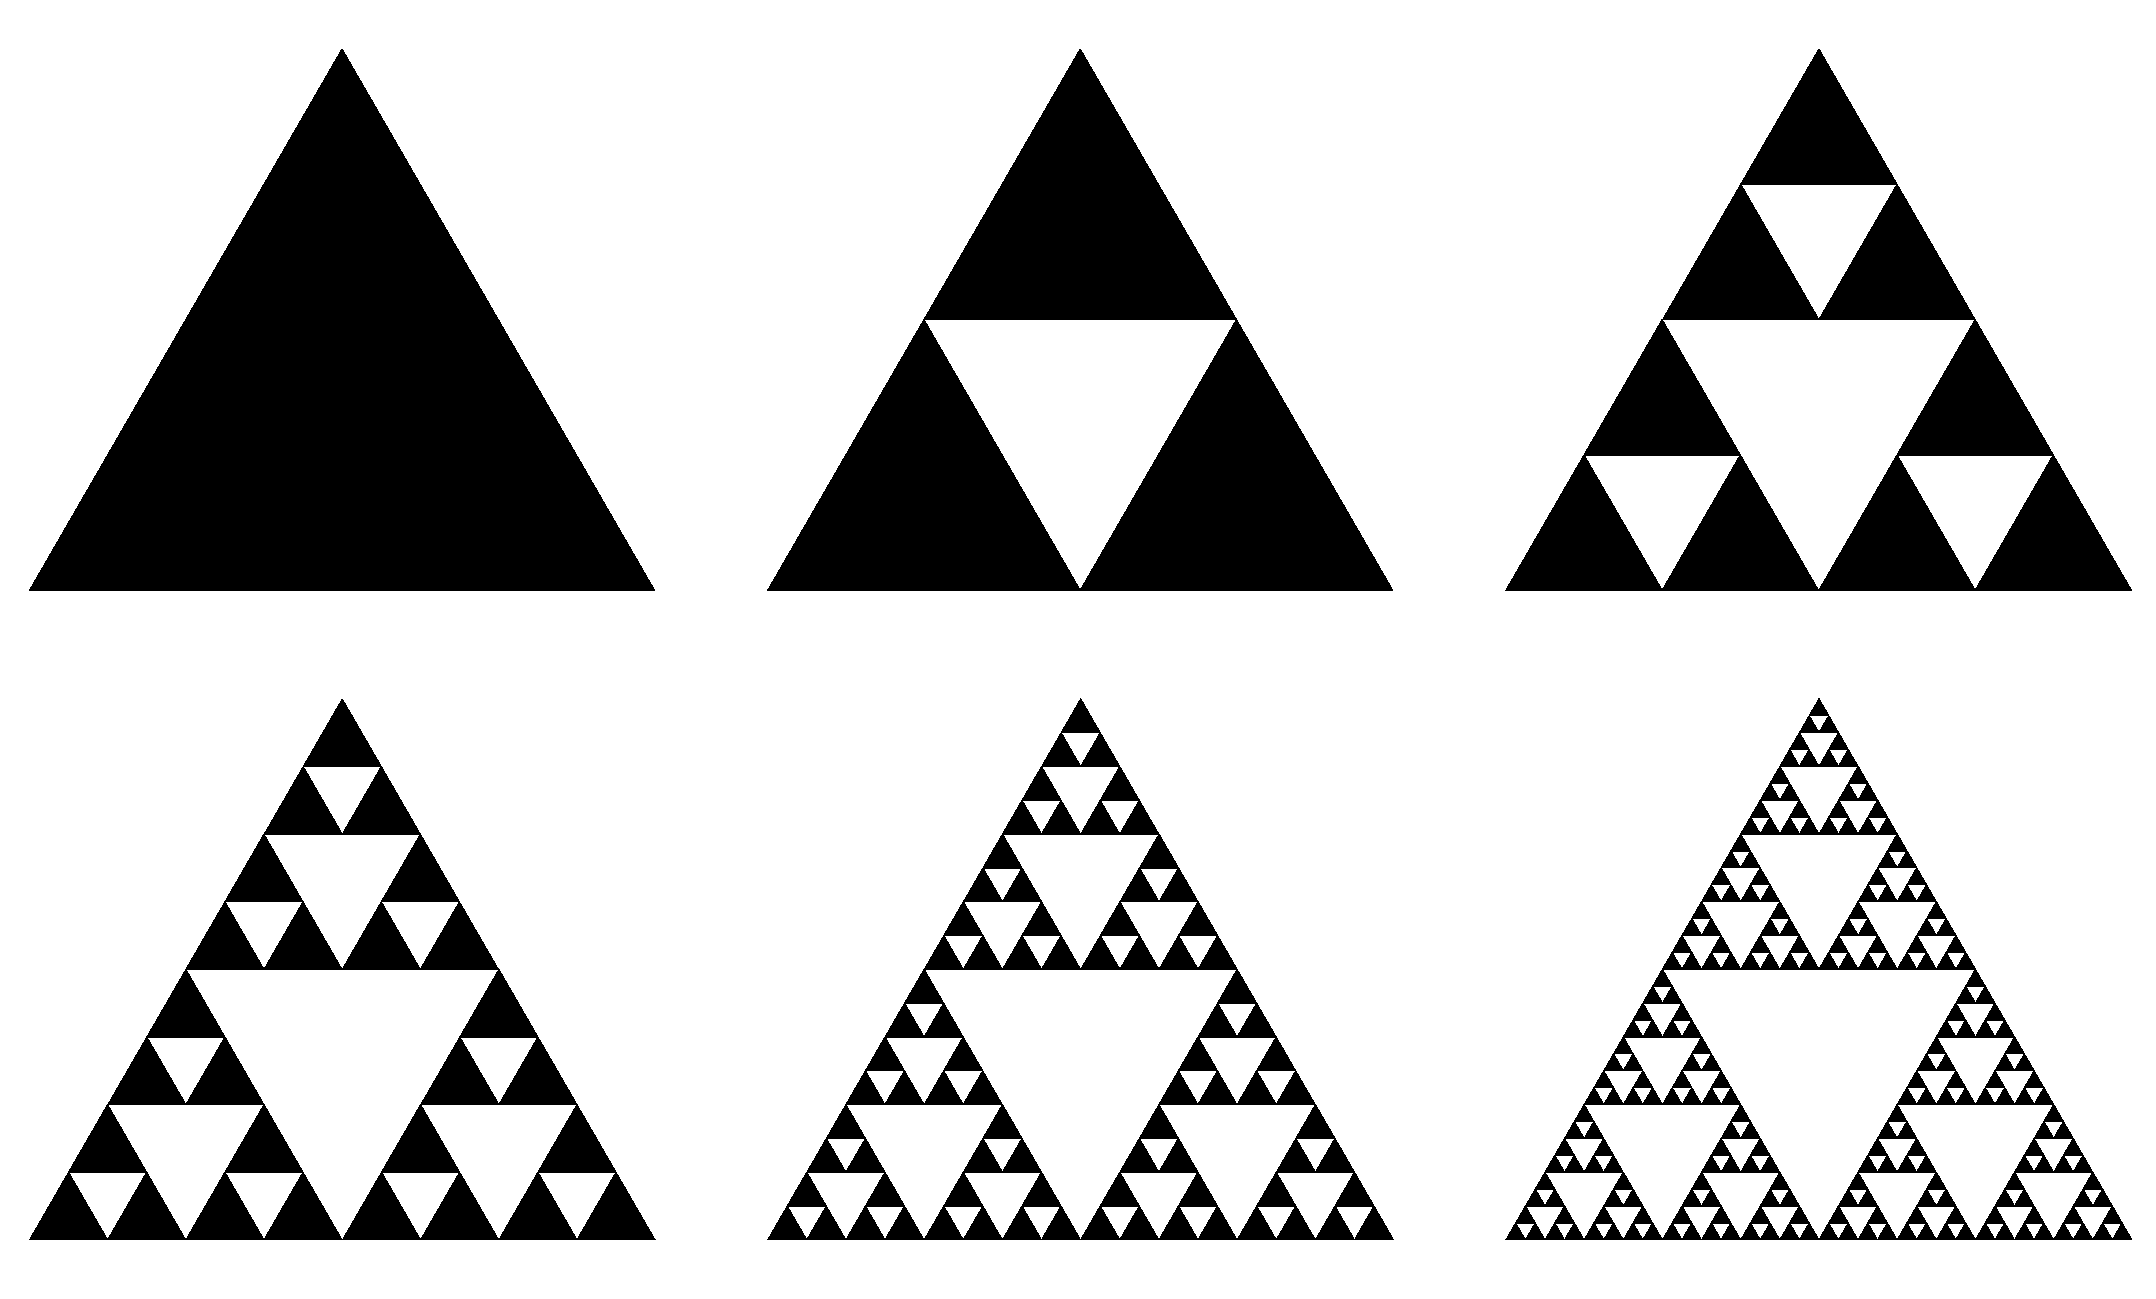
\includegraphics[width=(\imgWidth/2)]{images/sierpinski_triangle.pdf}
    \caption{Konstruktion eines Sierpinski Dreiecks.}
    \label{fig:sierpinski_triangle}
\end{figure}

Ein Fraktal ist ein geometrisches Objekt, das eine selbstähnliche Struktur aufweist. D.h. es sieht auf verschiedenen Skalen ähnlich oder identisch
aus. Das bedeutet, dass ein Teil des Fraktals eine verkleinerte Kopie des gesamten Fraktals ist. \cite{19_mandelbrot} Ein sehr bekanntes Beispiel
für eine solche Struktur ist das Sierpinski Dreieck. Dieses kann aus einem gleichseitigen Dreieck konstruiert werden,
indem man dieses mit drei kleineren gleichseitigen Dreiecken mit der halben Kantenlänge ersetzt, wobei in der Mitte eine Lücke entsteht. Ersetzt man
die neu enstandenen Dreieck immer wieder bis in's Unendliche nach dem gleichen Vorgehen, so ensteht das Sierpinski Dreieck. Die ersten paar Schritte
dieses Konstruktionsprozesses sind in Abbildung \ref{fig:sierpinski_triangle} zu erkennen. \cite{37_sierpinski} Eine simple Ersetzungsregel ermöglicht
hier das Bilden einer komplexen Struktur und kann technisch recht trivial mittels eines rekursiven Algorithmus umgesetzt werden. Fraktale lassen
sich häufig in der Natur wiederfinden, so z.B. in Schneeflocken, Küstenlinien, Wolken oder Pflanzen wie Brokkoli und Farnen, welche also algorithmisch
erzeugt werden können. \cite{19_mandelbrot}

\subsection{L-Systeme}
% ähnlich zu Fraktalen, ...

\subsection{Perlin Noise}
% gleiches Ziel wie Fraktal-Algorithmen
% diese jedoch sehr ineffzient, daher Verbesserung benötigt: Perlin Noise (Quelle 24: 2.2)
% Definition aus altem Grundlagenkapitel übernehmen und anpassen

\subsection{Zelluläre Automaten}



% l-systeme und zelluläre Automaten vllt zuerst vorstellen (chronologische Reihenfolge beibehalten)

\section{Inverse Verfahren}
% bis jetzt vorgestellte Verfahren hatten alles etwas gemeinsam: es wurden aufgrund von vordefinierten Regeln komplett neue Strukturen erzeugt
% -> inverse Ansätze gehen anders vor
\subsection{Model Synthesis}
% Merrell, Quellen 20-22
\subsection{Nutzen von partieller Symmetrie}
% Bokeloh et al., Quelle 3
\subsection{Wave Function Collapse}
\subsection{Inverses Ableiten einer Graph-Grammatik}
% Merrell, Quellen 1-2
